\chapter{Results}
\label{chap:simulation_results}

In this chapter, we present results for the estimation of actuation configuration for using both simulation data and data from the real system.
Since the parameter space of the motor orientation is not very intuitive, we transform the parameter results (and its variance) to a more intuitive form such that we can compare them.
One possibility would be to express the motor position in the Cartesian blimp frame $b$.
But since the position of the motor on the hull has only two degrees of freedom, a representation in the three dimensional blimp frame is not that much more intuitive.
A good solution is to represent the estimated motor position in the coordinate frame of the motor at its \textit{true}\footnote{
Since the true position is not known for real system results, we define one estimate as being true (e.g. the mean over all available estimates).
}
position, i.e. a coordinate system that is tangential on the sphere.
Then we can compare the multiple estimates in this \textit{tangential coordinate frame} $t$.
\\
The error of the actuator arrangement is expressed by an error distance $e_{pos}^k$ for each motor $k$, which is approximated by the euclidean norm in the x-y plane of the tangential frame,
and an error angle $e_{angle}$, which is the angle between x-axes of the 'true' and estimated motor coordinate systems $\mathbf{e}_{m_k}^x$ and $\mathbf{e}_{t_k}^x$.

\begin{figure}[hbtp]
\centering
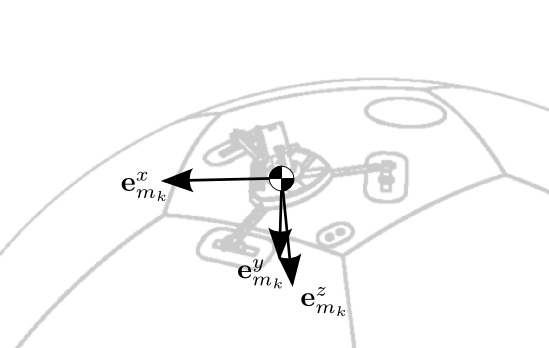
\includegraphics[scale=1]{images/tangential_frame.png}
\caption{The \textit{tangential frame} is the coordinate frame of the motor at its \textit{true} position. If the true position is not known, an estimate is used. In any case, its $\lbrace \mathbf{e}^x_{m_k} , \mathbf{e}^y_{m_k} \rbrace$ plane will be tangential to the spherical hull such that an error of the arrangement can be approximated by the euclidean norm in the tangential coordinate frame.
DRAW DISTANCE AND ANGLE INTO IMAGE. INCREASE RESOLUTION. CORRECT COORDINATE LABELS.}
\label{fig:tangential_frame}
\end{figure}

\section{Data used to generate Results}
To be able to generate meaningful results we recorded a long data set with Skye which contains about 850 seconds of undisturbed data samples.
To improve the accuracy of statistical results bootstrapping is applied to this large dataset.
Moving block bootstrapping is applied because the dataset consists of time series data. (??cite??)
The block stride is selected such that the dataset is divided in about 16 blocks.
Using 16 samples to calculate standard deviation values for the results 
According to margin of error (??cite??) calculations, the certainty that the actual standard deviation lies within 25\% of the standard deviation of the results from 16 blocks is 95\%.

\section{Simulation}
To test our optimization framework, we defined five test cases.
\begin{itemize}
\item[Default] A simulation of Skye blimp that is comparable to the real Skye system. All 21 parameters as listed in \cref{tab:params_updated} are estimated.
\item[1 AU] As default, but only one of the AUs of Skye is estimated (AU 4). The remaining AUs are not powered at all. 12 parameters estimated.
\item[5 AU] Different Skye blimp with 5 AUs. Configuration for all AUs estimated. 24 parameters.
\item[No Drag] As default, but simulation without aerodynamic drag. This is used to see how much drag influences the result accuracy.
\item[COG] As default, but with large additional weight at AU4 position. COG to COB offset is 10cm and yields a moment in the same magnitude as the actuation moment. This is used to estimate the error introduced by large COG shifts.
\end{itemize}
\subsection{Estimation Confidence}

\begin{figure}[hbtp]
\centering
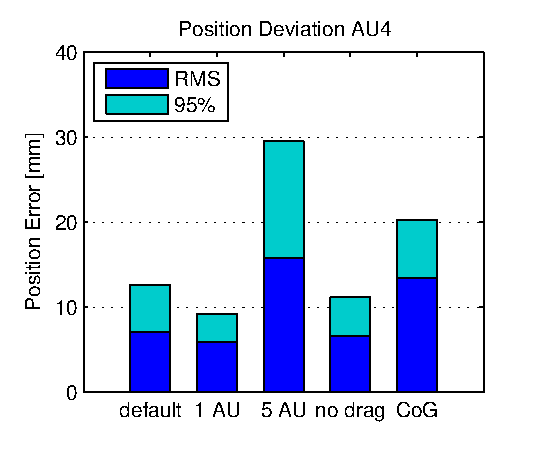
\includegraphics[scale=.72]{images/results/err_cmp_sim_pos.eps}
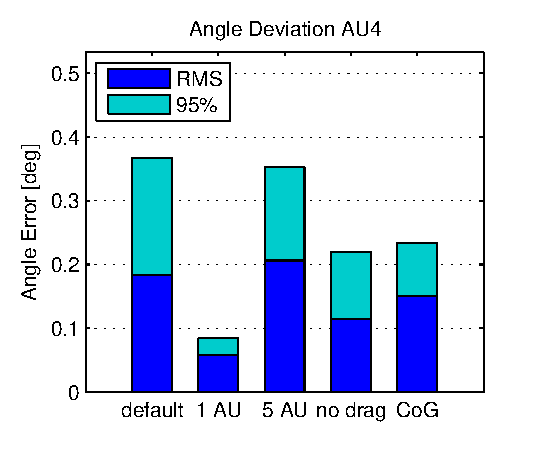
\includegraphics[scale=.72]{images/results/err_cmp_sim_angle.eps}
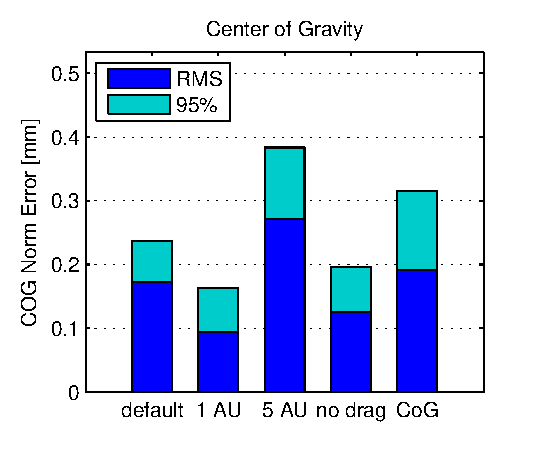
\includegraphics[scale=.72]{images/results/err_cmp_sim_cog.eps}
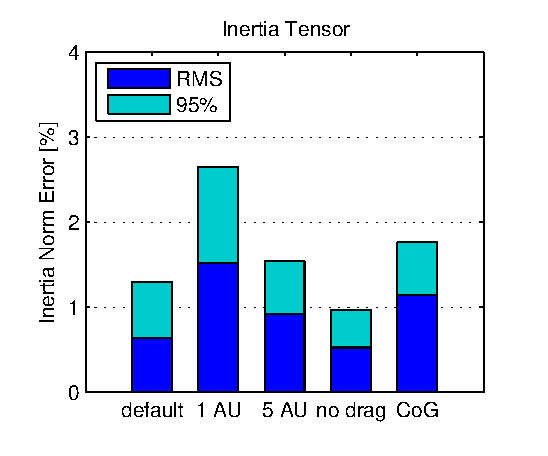
\includegraphics[scale=.72]{images/results/err_cmp_sim_tensor.eps}
\caption{Results for simulator}
\label{fig:err_cmp_sim}
\end{figure}



...Show estimate STD: BAR PLOTs.\\
...Similar explanations as in Presentation

\begin{figure}[hbtp]
\centering
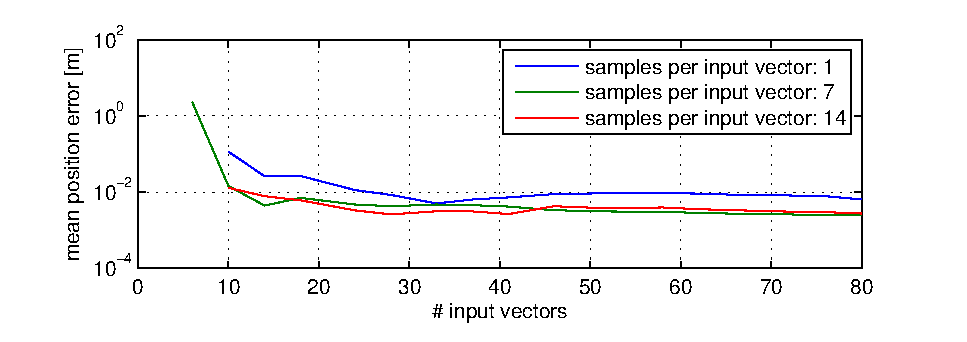
\includegraphics[width = \textwidth]{images/results/input_length_vs_position_error.eps}
\caption{Influence of the data set length on the mean position estimate error of the four AUs $e_{pos}$.}
\label{fig:result_inputlength}
\end{figure}

The confidence about the parameter estimates can be calculated as stated in \cref{sec:confidence_region}.
Nevertheless, the statistics can also been accessed by repeat the batch optimization using independent realizations.
\Cref{fig:result_95pc_confidence} shows the resulting position estimate for multiple realizations.
It can be seen that the 95\% confidence region calculated according to \cref{eq:variance_coordinates_tangential} (dashed line) well matches the 95\% confidence region calculated as $1.96$ times the standard deviation of the multiple realizations.
When calculating the standard deviation by \cref{eq:nlls_covariance}, it is crucial that the data for the batch optimization is independently drawn.
For us, that means that no more than one datapoint sample must be considered with the same input vector.
If multiple datapoints with the same input vector are drawn, the calculated standard deviation gets overconfident.
Hence, the results in \cref{fig:result_95pc_confidence} were calculated with only one datapoint per input vector\footnote{
As mentioned above, we splitted the available data into 16 subsets with 24 different input vectors each. Only one sample per input vector was used for this batch optimization.}.

\begin{figure}[hbtp]
\centering
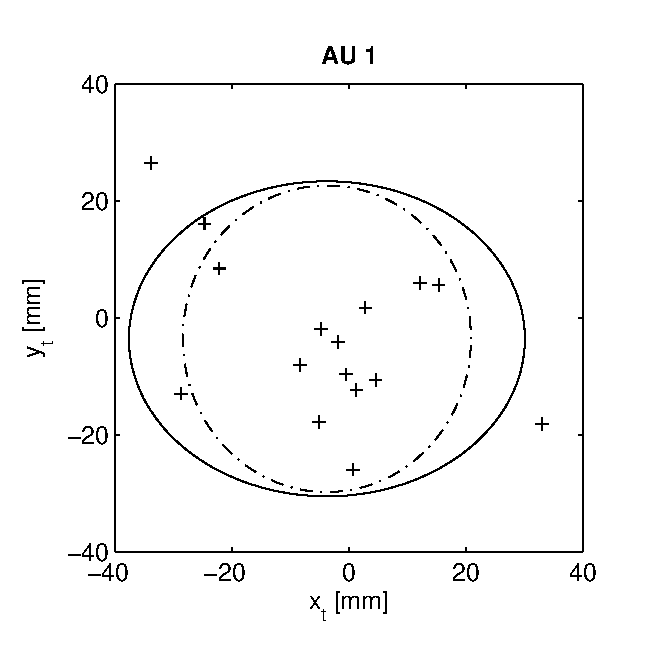
\includegraphics[width = 0.45\textwidth]{images/results/confidence_95_interval_AU1.eps}
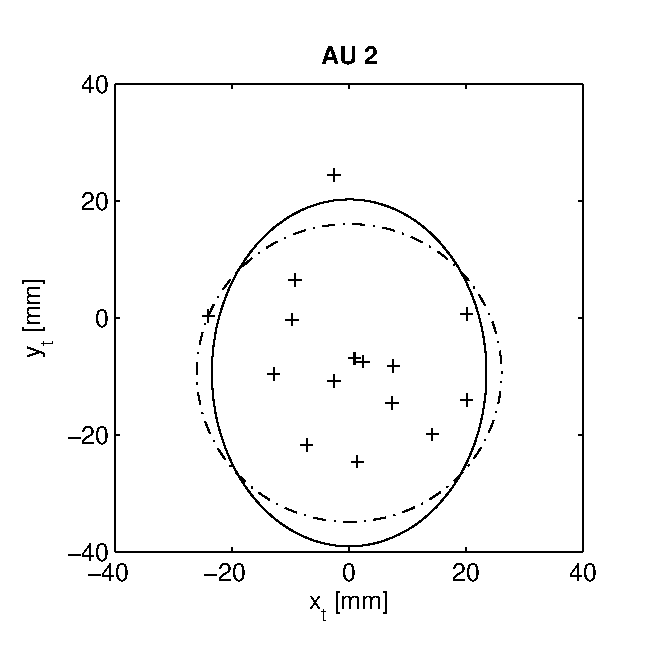
\includegraphics[width = 0.45\textwidth]{images/results/confidence_95_interval_AU2.eps} \\
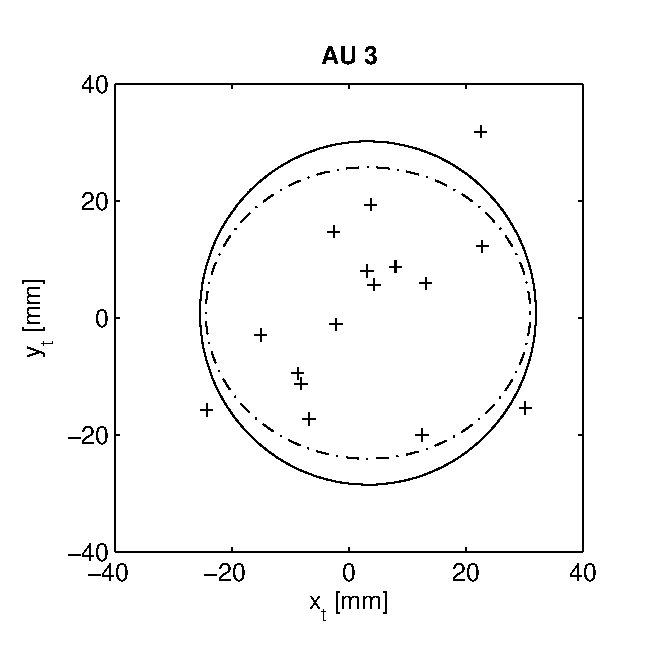
\includegraphics[width = 0.45\textwidth]{images/results/confidence_95_interval_AU3.eps}
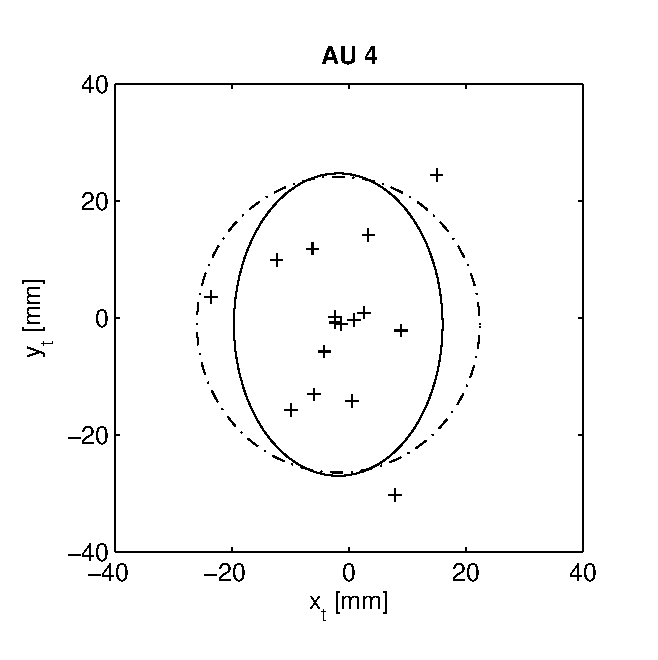
\includegraphics[width = 0.45\textwidth]{images/results/confidence_95_interval_AU4.eps}
\caption{Distribution of motor position estimates. $\mathbf{+}$: Realization. \textbf{solid}: 95\% confidence interval. \textbf{dashed}: 95\% confidence interval by residual.}
\label{fig:result_95pc_confidence}
\end{figure}



An important observation can be made about the influence of the dataset length on the estimate error.
\Cref{fig:result_inputlength} shows the change of error with increasing length of the dataset.
The more different input vectors are used for the batch optimization, the better gets the estimate.
When using multiple samples of the same input vector (in \cref{fig:result_inputlength} shown for 1, 7, and 14 samples per input vector), the estimation error decreases as well.
It can be seen that considering multiples of the same input vectors alone is not sufficient, to get a better estimate.
Varying the input is at least that important.

\subsection{Convergence Regions}
The impact of the initial estimate for the batch optimization has been tested.
Using different a grid of different initial configuration estimates, the failure rate for different input realizations has been tested and is shown in \cref{fig:result_sim_convergece_region}.
It can be seen, that a initial position offset of \textit{all} motors in any random direction\footnote{
The simulated blimp has a hull radius of \unit[1.37]{m} and therefore the distance between two of the tetrahedrally arranged actuation units is \unit[2.62]{m}.}
is acceptable up to \unit[1]{m}.
Initial orientation offsets of the motors are acceptable up to \unit[120]{°}.
\\
The same observation can be made when using datasets from real measurements (compare \cref{fig:result_real_convergece_region}).
Further results using real measurements are showed in the next section.

\begin{figure}[hbtp]
\centering
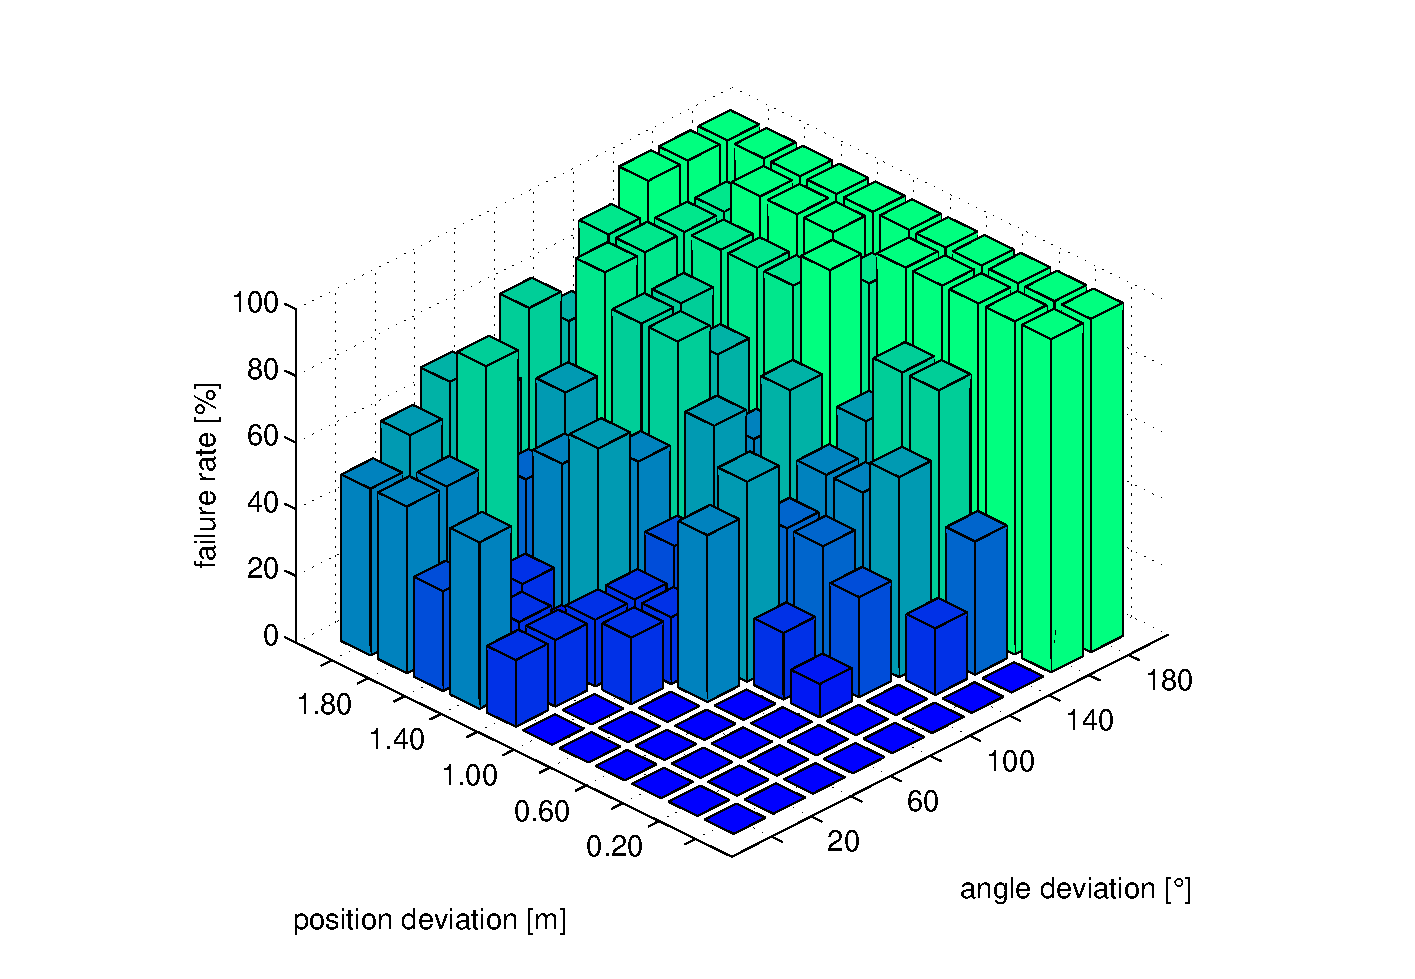
\includegraphics[width = \textwidth]{images/results/convergence_analysis_init_deviation_sim_bar.eps}
\caption{Failure rate using simulation data and different initial guess about actuation configuration.}
\label{fig:result_sim_convergece_region}
%\end{figure}
%
%\begin{figure}[hbtp]
\centering
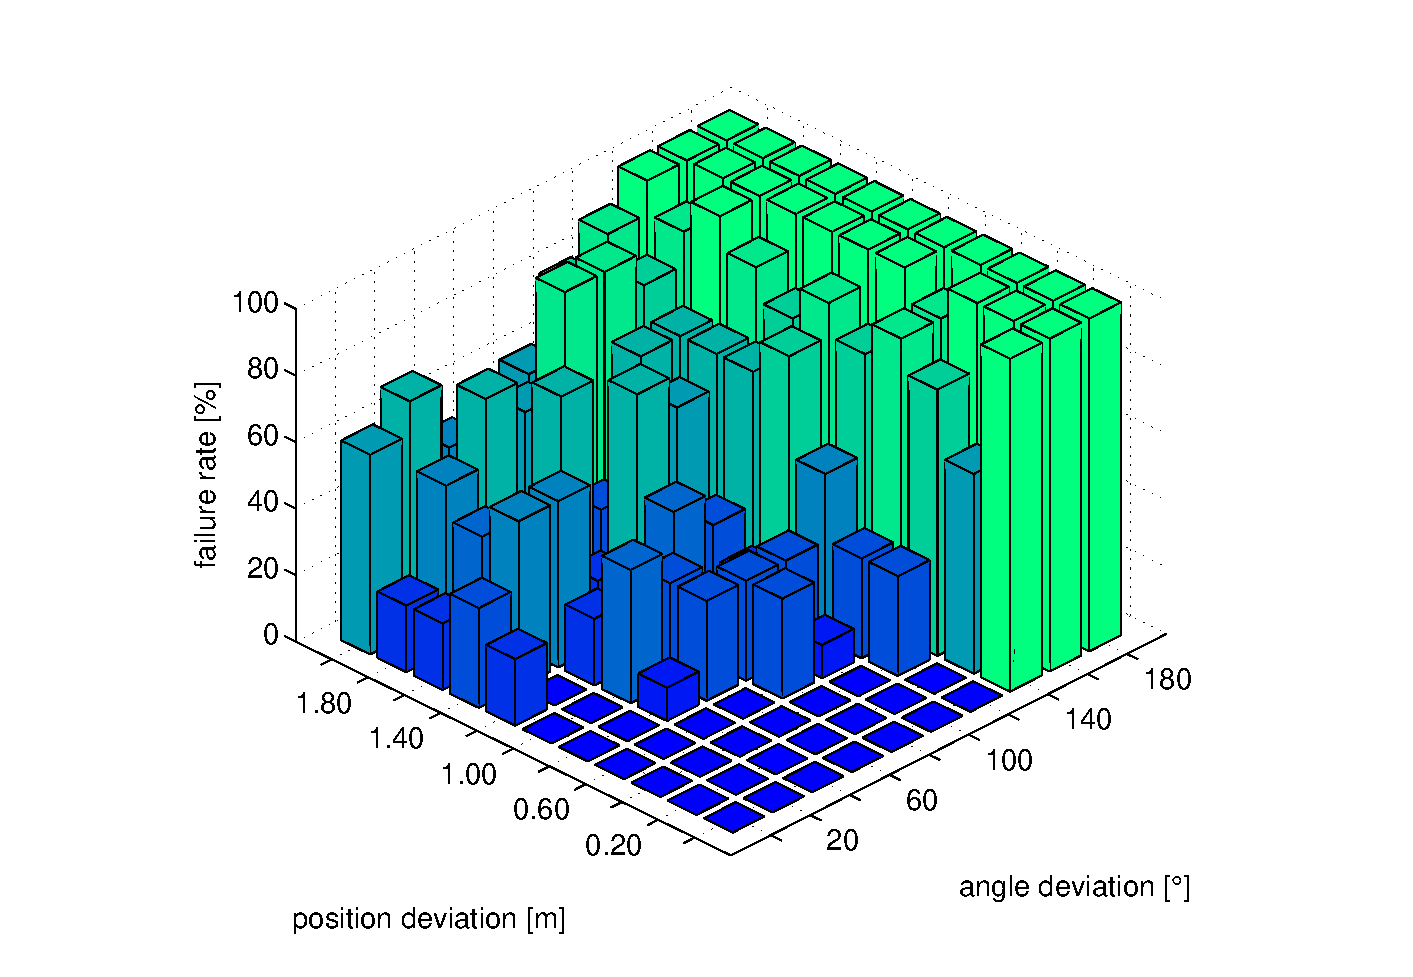
\includegraphics[width = \textwidth]{images/results/convergence_analysis_init_deviation_real_bar.eps}
\caption{Failure rate using experiment data and different initial guess about actuation configuration.}
\label{fig:result_real_convergece_region}
\end{figure}


\section{Experiments}
\subsection{Estimation Confidence}
...Copy past from Simulation. Replace STD by RMS. Compare Experiment with Simulation.
...That means do not show a 'you-know-which-plot' again (it will be very similar to the one above)
...But show this angular acceleration plot. Add a error subplot to it.
\subsection{Convergence Regions}

\begin{figure}[hbtp]
\centering
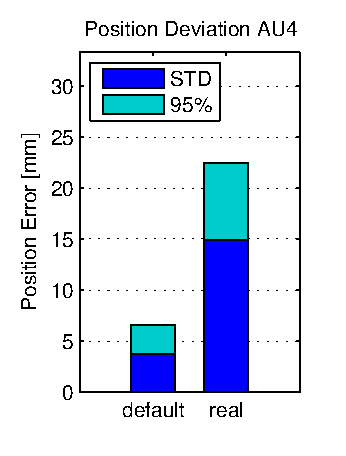
\includegraphics[scale=.72]{images/results/err_cmp_real_pos.eps}
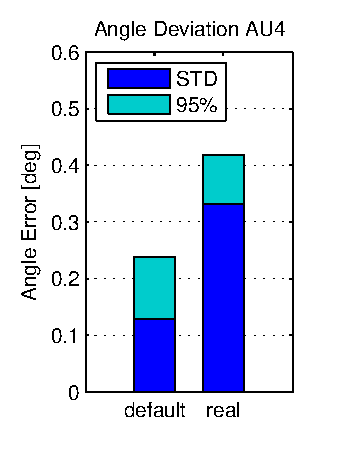
\includegraphics[scale=.72]{images/results/err_cmp_real_angle.eps}\\
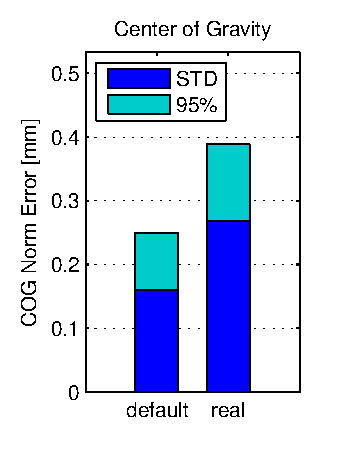
\includegraphics[scale=.72]{images/results/err_cmp_real_cog.eps}
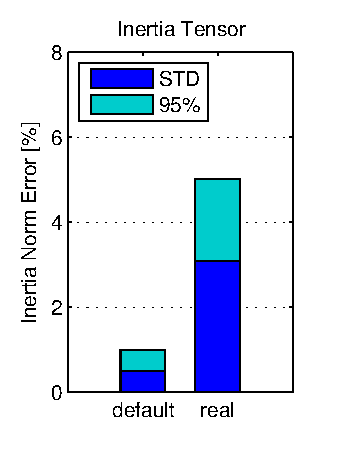
\includegraphics[scale=.72]{images/results/err_cmp_real_tensor.eps}
\caption{Results for real system}
\label{fig:err_cmp_real}
\end{figure}


\section{Ground Truth}
...Do not tell toooo much in this section. Nobody likes to read long reports. So just mention 'we did it' and show the results.

...